\documentclass{article}
\usepackage{graphicx} 
\usepackage{amssymb}
\usepackage{amsmath}
\usepackage{algpseudocode}
\usepackage{caption}
\usepackage{graphicx}
\usepackage{caption}
\usepackage{subcaption}
\usepackage{dingbat}
\usepackage{amssymb}
\usepackage{algorithm}
\usepackage{algpseudocode}
\usepackage{amsmath}


\title{Project Report \\ CUDA Theta*}

\author{Robert Fischer }

\begin{document}

\maketitle

\section{Introduction}
%
This report aims to summarize the Theta* project. Please forgive any spelling mistakes, I wrote this report under very tight time constraints. Also note, also due to time constraints, there slipped in an error where the absolute runtime durations were incorrectly reported. Hence, only consider relative runtime durations.
%
\section{Map generator}
%
Theta* is a pathfinding algorithm which operates on any cost-graph $(N, C) \in G$ for which a heuristic function $h(x_0,y_0,x_1,y_1)$ exists, which heuristically determines the assumed cost left to reach the goal $(x_0,y_0) \in \mathbb{R}^2$. $(n_x, n_y) \in N \in \mathbb{R}^2$ represent the nodes of the graph $G$ the  $((x_0), (y_0), (x_1, y_1) \in C \in \mathbf{R^2}\times\mathbf{R^2}$ represent the connection for the graph $G$. Each node has an obstacle property $O(n)$ which is $1$ if it is solid and not passable and $0$ if it is passable. In order to evaluate my approach I created a procedural map-generator. The map-generator generates square $NxN$ sized 2D grids where $O((x,N - 1))=1$, $O((x,0))=1$, $O((N - 1,y))=1$ and $O((0,y))=1$, i.e. the borders are closed. Additionally, I place $K$ uniformly sampled, random rectangles with maximum random width and height between 1 and 10 tiles. This results in maps looking similar to Figure~\ref{fig:map_gen}.
%
\begin{figure*}[h]
    \centering
    \begin{subfigure}[b]{0.49\textwidth}
        \centering
        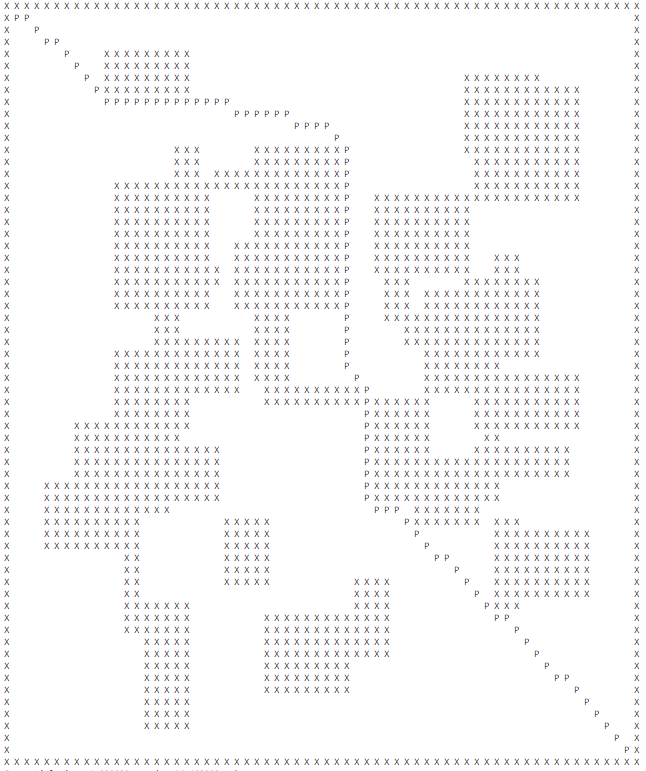
\includegraphics[width=\textwidth]{figures/map_1.png}
    \end{subfigure}
    \begin{subfigure}[b]{0.49\textwidth}
        \centering
        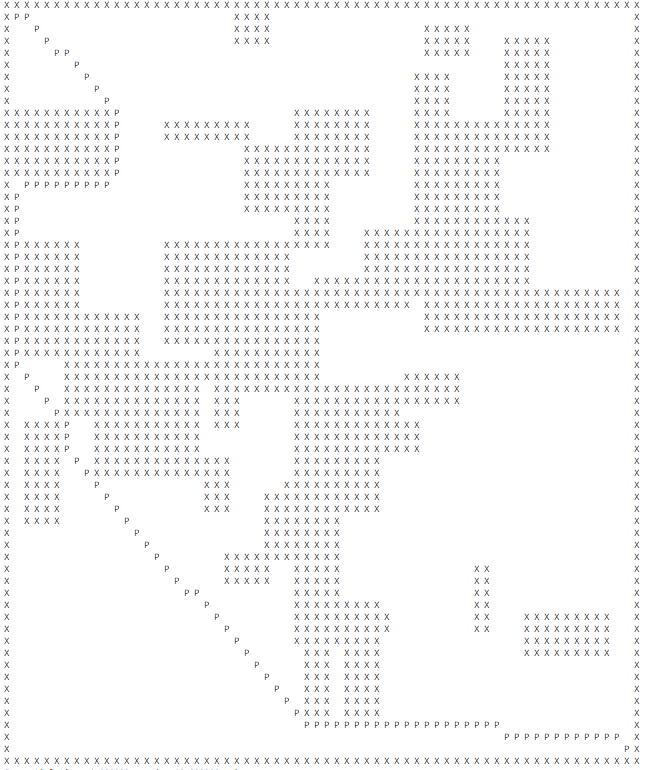
\includegraphics[width=\textwidth]{figures/map_2.png}
    \end{subfigure}
    \begin{subfigure}[b]{0.49\textwidth}
        \centering
        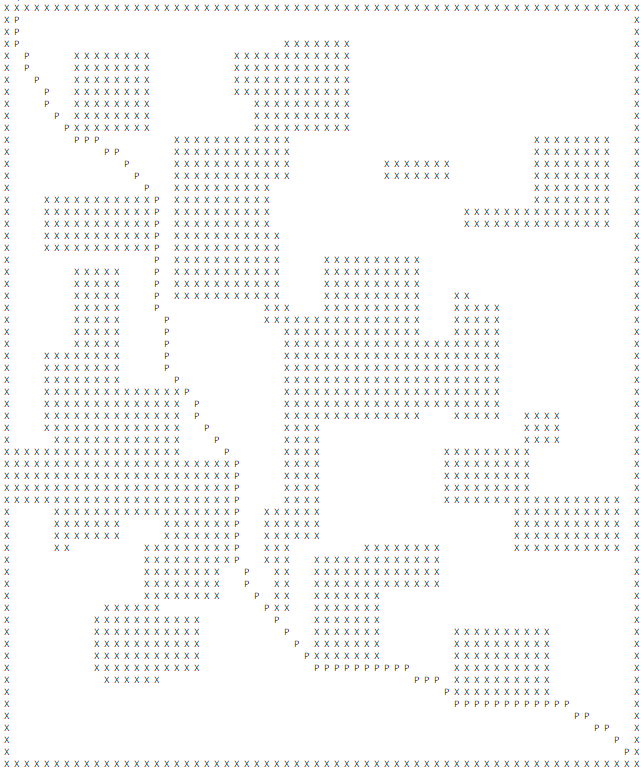
\includegraphics[width=\textwidth]{figures/map_3.png}
    \end{subfigure}
    \begin{subfigure}[b]{0.49\textwidth}
        \centering
        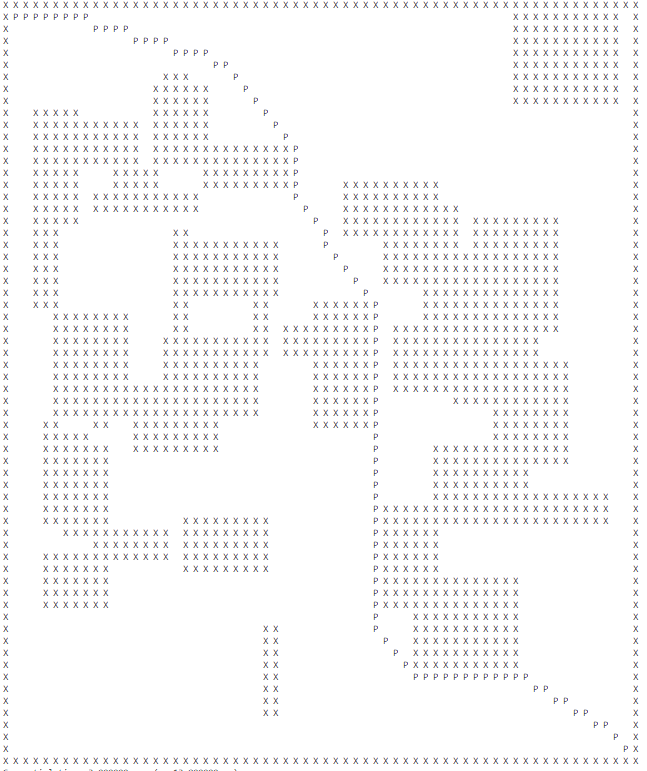
\includegraphics[width=\textwidth]{figures/map_4.png}
    \end{subfigure}
    \hfill
    \caption{Sample maps generated by the map generator.}
    \label{fig:map_gen}
\end{figure*}
%
\section{Sequential Implementation}
%
In order to evaluate the relative speed-ups I implemented an A* path-finding algorithm and extended it with the Theta * path extension rule. The main difference between A* and (Basic) Theta* is that, if there exists a straight line between an expanded node and their parent, the node which is used for extension is "skipped" and the parent of the new entry in the open list is the current node's parent. Resulting in more natural looking paths, but also losing the property that Theta* finds the most optimal path. Instead, it finds relatively good looking paths.

In order to determine the visibility of two nodes, I implemented an integer-based Bresenham algorithm. Problem encountered here, was that it sometimes happened that paths which were found "slipped" through certain gaps. This was fixed, by considering checking a 2x2 area per bresenham iteration (i.e. $(x,y)$, $(x+1,y)$, $(x,y+1)$ and $(x+1,y+1)$).

The most important data structure for Theta* is the priority queue. For the priority queue I use boost::container::priority\_queue with a red-black balanced tree as a backend data structure. It allows most important operations in O(log n) (insert, extract, replace, etc.). Theta* additionally requires fast positional access (due to it's replacing nature), hence I added an additional "shadow" data structure with the position as query.
%
\section{Theta* with grid as replacement for priority queue}
%
This section outlines how the experiment where we replace Theta*'s priority queue through an implicit gird-based representation
%
\subsection{General}
The goal of this approach was to investigate a more creative solution of creating a paralellized implementation of Theta*. The main insight of this solution is that A* mainly operates locally (neighboars of the grid), so I can parallelize A* by applying kernels on the grid with an offset of 3 along the x- and y-axis in parallel.
\begin{algorithmic}

\State $S \gets \text {number of tiles in map}$
\State $BS \gets \text {block size of kernel}$
\State $O \gets \{(0, 0), (1,0), (2,0), (1,0), (1,1), (1,2), (2,0), (2,1), (2,2)\}$
\While{Any tile open?}
\For{$(o_x,o_y) \in O$}
\State \textbf{Kernel}$[S/BS/3+1, S/BS/3+1), (S / BS / 3 + 1),(BS, BS))]$($o_x$, $o_y$)
\State \textbf{Synchronize}()
\EndFor
\State Write \textbf{Write Only} data to \textbf{Read Only}
\EndWhile
\end{algorithmic}
Hence, this \textbf{Kernel} allows the execution of $1/9$th of the grid's in parallel. Most tiles will most likely not have any occupancy of the algorithm (hence, they execute pretty fast). This could also be improved by applying a prefix sum to determine the "occupied" tiles and execute the kernel only on those tiles directly.
%
\subsection{Main Kernel}
%
The kernel itself is pretty similar to the A* inner loop: Each tile, checks first  if it is "open". If no, skip this tile. If yes, continue. Then, if I have already found a valid path to the goal position, it checks if the cost of the found path $f_1$ of this tile is worse than the already found best cost $f_2$ of current tile and if so, the current tile openness is set to $0$ again.

Next I check, if the current tile is the goal tile, if so, I store this information using atomic CUDA operations: whether I found any goal and the exact cost $f$ to reach the goal (minimum of current best cost and new found best cost).

I also set the closed flag to $1$, so I know this tile has been visited. I tested several variants where the closed flag was only set under certain conditions: i.e. only close if surrounding neighbors have been opened or never close (as it might be relevant in the future), or only close if cost is below best candidate.

I then expand the neighbors according to the A* and Theta* rules. For the Theta* extension rule, with the added change that for the Theta* rule I set the closed property of the neighbor, current and parent nodes to $0$ again. This means they are considered again for future iterations again.

Also to ensure that there are no concurrent write operations while executing the kernel, the relevant data structures are put into \textbf{read-only} and \textbf{write-only} memory. The read-only memory is only read from the kernel and the write-only memory is only written to from the kernel. After executing all kernels, I then synchronize the read-only data with the write-only data by copying the respective memory.

This algorithm could be summarized, in the following way: it works similar to flood-fill, but, I weight using the cost-functions the possible paths and determine using this technique if I reached the goal or not.
%
\subsection{Maximum cost by reduction}
%
Crucial part of this approach is to determine if the algorithm has already found the best solution available. To achieve this, I implemented a global reduction which calculates the current best-cost by reducing the maximum cost over all tiles. Any tile, which is worse than that, can be skipped. Reduction can be seen similar to how Mip-mapping works (mean over texture) in computer graphics: essentially, first the operation is applied locally and then gradually repeated over wider ranges based on previous results. I learned it is quite difficult to get it to work correctly and fast.
%
In the end, this was not necessary, as atomic operations showed to be easier to handle and more performant (no additional kernel execution required).
%
\subsection{Ping-pong buffers}
%
I also tried to optimize away the final memory synchronization by swapping the read-only and write-only buffers each iteration, i.e. the previous read-only data structure becomes write-only and vice versa. In theory, this meant that much less data copying is required. In practice, I did not manage to achieve this without breaking the algorithm to find proper paths.
%
\section{Theta* with distributed priority queues}
%
This section outlines a more direct Theta* port to CUDA.
\subsection{General}
%
The main inspiration for this implementation comes from Zhou \textit{et. al} \cite{Zhou15}. Their approach introduces $N$ independent priority queues. Those queues are extracted from and expanded independently into a list $S$. This list is then deduplicated, where we remove nodes which have already been found twice (or more) by multiple priority queues. Then the remaining nodes are distributed again between the priority queues.

The paper does not tell much about specific implementation details, especially the node duplication is quite tricky and also leaves some very important things out (i.e that the node de-duplication should not only consider the closed list, but also the states within the open list). The priority queue data structure is a min-heap. The states are stored in a state-pool.

The code works as follows: first we add the starting node to the first priority queue. Then we reset all relevant memory. Then we execute the ExtractAndExpand kernel, which essentiall runs each priority queue in parallel. For each priority queue, the minimum cost node is removed, and the potential neighbors are added to a list S. Potential neighbors are candidates, which do not collide with the terrain and which satisfy the Theta* and A* conditions.

We then check if we have reached the goal and the current best cost is the best cost node within all open lists. If so, we terminate and return the found path.

After filling the list S, we filter using duplication detection. More details in the next section. Once the filtered list T is available, I distribute the remaining nodes two the different priority queues. What is not written in the paper, but is crucial is to add a value which is constantly increased with each iteration (i.e. (queue\_idx + iteration) MOD NUM\_QUEUES). This can be done efficiently through the use of \_\_syncthreads() function of CUDA.
%
\subsection{Duplication detection}
%
The main challenge with the implementation was the duplication detection. After filling the list S, we construct a filtered list T. The list T does not contain any duplicates from the closed set and no duplicates within itself. This is achieved by 2 kernels. The first kernel checks the existing closed nodes, and filters if there already exists a better closed one. Filtering means that we assign a binary 1 if it is relevant or 0 if it is not relevant. And while iterating through the list, we store, using atomics, the lowest cost per position (x,y) in a 2D array. With the next kernel, we again iterate through the filtered binary list, but here we additionally check if the cost of the node is lower or equal to the lowest cost node found in the previous kernel.

Having this binary mask, we can then apply a prefix-sum which constructs the indices used. After the prefix-sum, we can then apply a final kernel which copies over the values to the filtered list T.
%
\subsection{Issue}
%
The main issue with my current implementation is that it does not find paths with the same length as the sequential implementation. I argue this is a bug somewhere within the code, but possibly could also be an artifact of Theta* being not guaranteed to find the best path. But, usually the parallel implementation finds worse paths, hence I lean more towards taht there is some bug in the code present.
%
\section{Performance analysis}
%
In this section, I outline my Theta* implementation over various modalities. Each experiment has been repeated 5 times. I report the median runtime duration (in milliseconds) and mean absolute difference from the median of measured runtimes (i.e. MAD) (in milliseconds). Additionally, I report the path length difference using $L_2$ norm, i.e. 0 means path is equivalent in length. The start position is always $(1,1)$ and the goal position is $(N-2,N-2)$.

The experiments run on a Google Colaboratory Pro instance using an Nvidia V100 GPU and an Intel Xeon CPU 2.20GHz with 25.5GB RAM.
\subsection{Number of priority queues}
\label{sec:prio_queue}
%
This experiment aims to investigate the impact of the different number of queues. For this experiment, I set the obstacle ratio to 35\%. The map size is $1024 \times 1024$ and I modulate the number of priority queues. There exists two parameters to adjust: the number of blocks $BN$ and the number of threads per block $TN$. The number of priority queues used by the implementation is $BN \cdot TN$. As the number of threads per block is not limited, I change the two parameters such that the number of queues match the desired values. In Table~\ref{tab:prio_queue} we observe that there exists a sweet-spot of priority queues for the aforementioned settings around 512 priority queues. Referring to Figure~\ref{fig:prio_queue}, I plotted the respective number of queues versus the median runtime duration. I expected the sweet-spot to be the highest number of threads per block, with the lowest number of blocks, as this means that the GPU's pipeline is fully used, without the additional management required for multiple blocks. 
%
\begin{table}[]
    \centering
    \begin{tabular}{|c|c|c|c|c|}
        \hline
        \textbf{BN} & \textbf{TN} & \textbf{No. Queue} & \textbf{Duration (ms)} & \textbf{MAD (ms)} \\
        \hline
        4 & 256 & 1024 & 596 & 2362 \\
        \hline
        3 & 256 & 768 & 575 & 2328 \\
        \hline
        \textbf{1} & \textbf{512} & \textbf{512} & \textbf{541} & \textbf{1808} \\
        \hline
        1 & 256 & 256 & 698 & 2743 \\
        \hline
        1 & 128 & 128 & 1128 & 4306 \\
        \hline
    \end{tabular}
    \caption{Comparing runtimes using different number of priority queues.}
    \label{tab:prio_queue}
\end{table}
%
\begin{figure*}[h]
    \centering
    \begin{subfigure}[b]{1.0\textwidth}
        \centering
        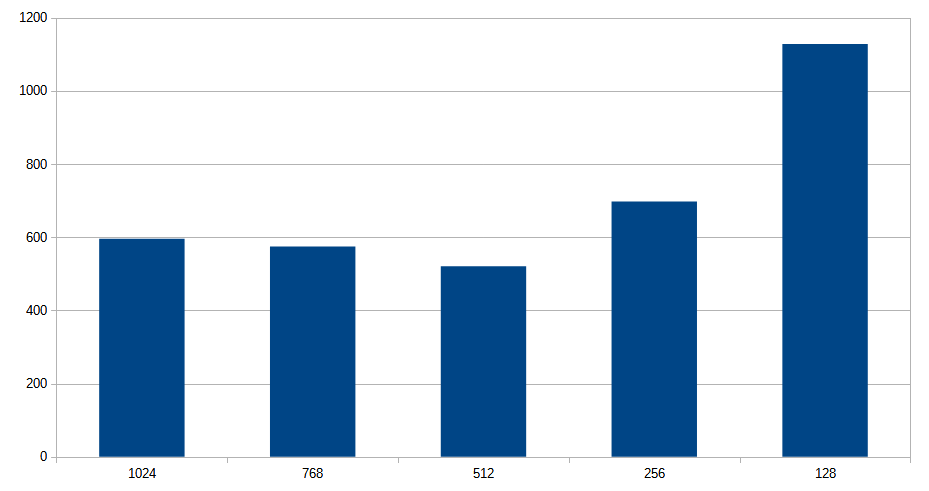
\includegraphics[width=\textwidth]{figures/prio_queue.png}
    \end{subfigure}
    \hfill
    \caption{Comparison of runtimes with different number of priority queues. Y-axis represent duration in milliseconds. X-axis represents number of priority queues used.}
    \label{fig:prio_queue}
\end{figure*}
%
\subsection{Map size}
%
In this experiment, I want to investigate how various map sizes influence the duration of the path-finding algorithm. I compare the performance of the sequential algorithm versus my CUDA implementation. I set the obstacle ratio to 35\% and set number of priority queues to 512 (based on the results of Section~\ref{sec:prio_queue}). We observe in Table~\ref{tab:map_size}, that in general the GPU implementation runs faster than the sequential implementation the larger the map (every map size beginning with 256). Interestingly, the resulting path length for the CPU implementation is also shorter than the GPU implementation. This could be due to an implementation bug in the CUDA code, due to the fact that Theta* is not guaranteed to find the shortest path and depends on the order of execution or another explanation could be that this is due to different floating point operations (and inaccuracies). Exact reason for this path length difference is not yet clear and requires further investigation. We also observe higher MAD values for sequential implementations, but this could be due to the sequential code running longer, leaving more possibility for the operating system to schedule different processes and hence higher variance in runtimes. Refer to Figure~\ref{fig:map_size} for comparing the differences visually. We observe that for larger map sizes the performance gain scales to a factor of 2-3x.
%
\begin{table}[]
    \centering
    \begin{tabular}{|c|c|c|c|c|c|}
        \hline
        \textbf{Size} & \textbf{Par. dur.} & \textbf{Sequ. dur.} & \textbf{Par. MAD} & \textbf{Sequ. MAD} & \textbf{$\Delta$Path len.} \\
        &[ms] & [ms] & [ms] & [ms] & \\
        \hline
        1536 & 1408 & 4294 & 5587 & 17030 & 2 \\
        \hline
        1024 & 541 & 1808 & 2170 & 7223 & 3.16 \\
        \hline
        512 & 124 & 416 & 482 & 1676 & 3.5 \\
        \hline
        256 & 42 & 93 & 172 & 378 & 0 \\
        \hline
        64 & 7 & 4 & 29 & 16 & 0 \\
        \hline
    \end{tabular}
    \caption{Comparing runtimes using different map sizes.}
    \label{tab:map_size}
\end{table}
%
\begin{figure*}[h]
    \centering
    \begin{subfigure}[b]{1.0\textwidth}
        \centering
        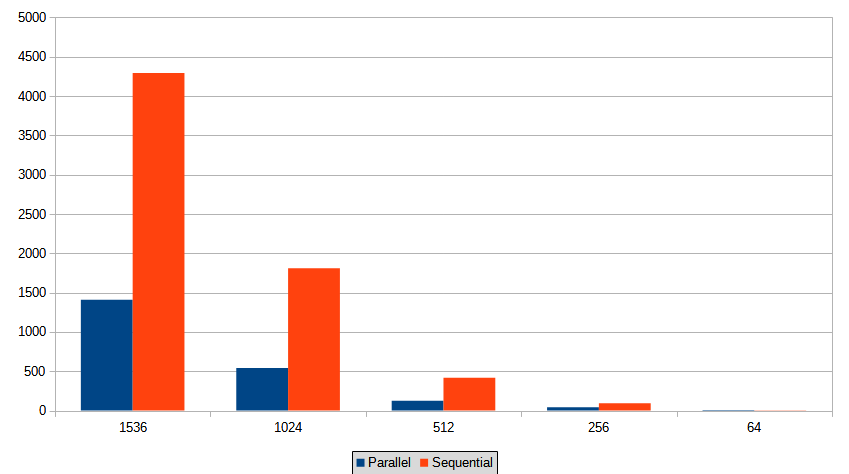
\includegraphics[width=\textwidth]{figures/grid_size.png}
    \end{subfigure}
    \hfill
    \caption{Comparison of various map sizes. Y-axis represent duration in milliseconds. }
    \label{fig:map_size}
\end{figure*}
%
\subsection{Map density impact}
%
In this experiment, I perform both sequential and parallel path-finding on maps with different percentage of tiles occupied i.e. different map densities. I assume three modalities: Sparse, normal and dense maps. Sparse maps are maps where 5\% of the tiles are occupied, normal maps have 30\% of tiles occupied and dense maps have 50\% of tiles occupied. Any more, means that sometimes the procedural generation creates maps which do not have a valid solution, which we do not consider for this experiment. The remaining evaluation parameters are kept similar to the other experiments (i.e. map size 1024, obstacle ratio 35\% and 512 priority queues).

In Table~\ref{tab:map_impact}, we observe that the runtimes for sparse maps (5\%) is longer than for the other modalities. I argue, this is due to the fact that in sparse maps there are potentially more open nodes and hence, more tiles need to be visited. Still, this is quite unexpected. We also observe that for 50\% the path length difference is relatively high. This is something which needs to be investigated further in the future, as it may be a bug in the implementation. We also observe that the parallelized implementation is still 2-3x faster than the sequential implementation in all cases.
%
\begin{table}[]
    \centering
    \begin{tabular}{|c|c|c|c|c|c|}
        \hline
        \textbf{Size} & \textbf{Par. dur.} & \textbf{Sequ. dur.} & \textbf{Par. MAD} & \textbf{Sequ. MAD} & \textbf{$\Delta$Path len.} \\
        &[ms] & [ms] & [ms] & [ms] & \\
        \hline
        5\% & 1847 & 3422 & 7436 & 13735 & 3.52 \\
        \hline
        30\% & 541 & 1808 & 2170 & 7223 & 3.16 \\
        \hline
        50\% & 569 & 1373 & 2284 & 5476 & 14.21 \\
        \hline
    \end{tabular}
    \caption{Comparing runtimes using different map densities.}
    \label{tab:map_impact}
\end{table}
%
\begin{figure*}[h]
    \centering
    \begin{subfigure}[b]{1.0\textwidth}
        \centering
        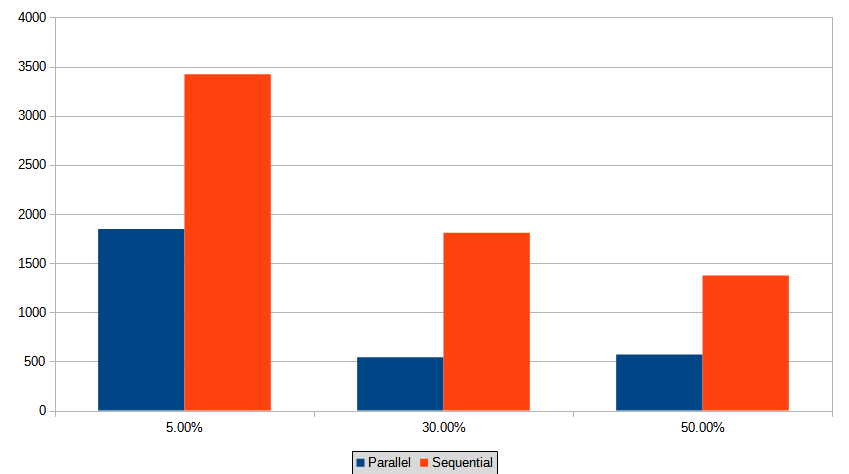
\includegraphics[width=\textwidth]{figures/map_density.png}
    \end{subfigure}
    \hfill
    \caption{Comparison of various map densities. Y-axis represent duration in milliseconds. }
    \label{fig:map_density}
\end{figure*}
%
\subsection{Map variance}
%
For this investigation, I evaluated the algorithm over different generated maps by using different random seeds. The remaining parameters are as usual (map size 1024, obstacle ratio 35\% and 512 priority queues). Refer to Figure~\ref{fig:map_variance} for a comparison between the sequential and parallel implementation's runtimes. We observe a relatively low variance of runtimes for both implementations, implying that different procedural maps have similar path-finding durations. However, in Figure~\ref{fig:map_variance_path}, we observe a high variance with regards to the found path length divergence, implying that the path error is map dependent.
%
\begin{figure*}[h]
    \centering
    \begin{subfigure}[b]{1.0\textwidth}
        \centering
        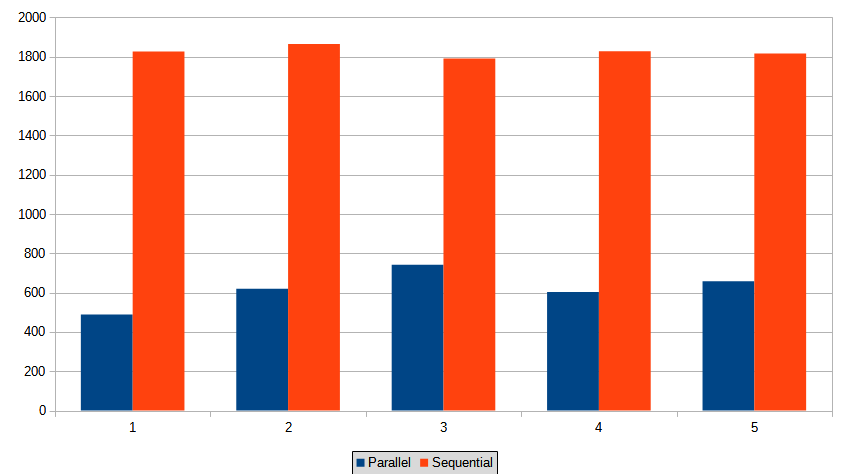
\includegraphics[width=\textwidth]{figures/map_variance.png}
    \end{subfigure}
    \hfill
    \caption{Comparison of path finding duration over different random seeds.. Y-axis represent duration in milliseconds. X-axis represents used random seed.}
    \label{fig:map_variance}
\end{figure*}
%
\begin{figure*}[h]
    \centering
    \begin{subfigure}[b]{1.0\textwidth}
        \centering
        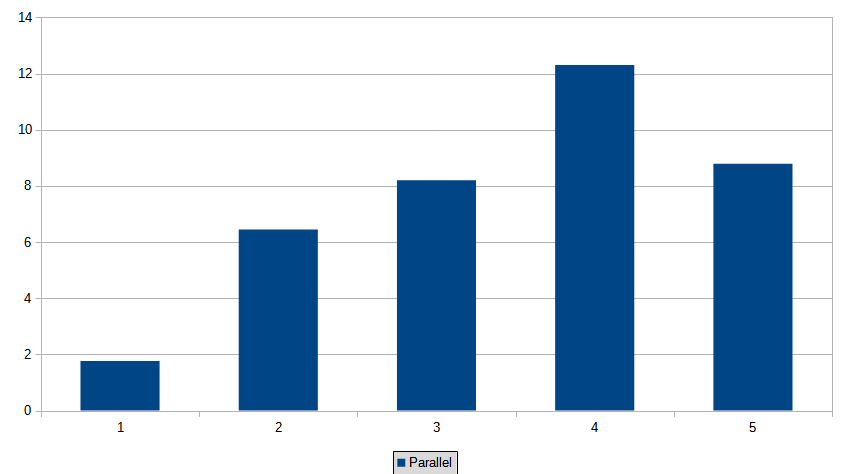
\includegraphics[width=\textwidth]{figures/map_length_diff.png}
    \end{subfigure}
    \hfill
    \caption{Comparison of path finding duration over different random seeds. Y-axis represent path length delta comparing the sequential and parallel implementations. X-axis represents used random seed.}
    \label{fig:map_variance_path}
\end{figure*}
%
\subsection{Memory strategy}
%
In this experiment, I evaluate the impact of different memory management strategies. The default cudaMemCopy based experiment (1024 map size, obstacle ratio 35\% and 512 priority queues) serves as a baseline for comparison with a pinned memory implementation and a zero-copy implementation. Both variants only apply those memory strategies for memory access patterns within the main algorithm loop, as the memory access outside this loop will be ammortized over execution time. In Table~\ref{tab:mem_strat}, we observe that pinned memory strategy slightly outperforms the other strategies, although the difference is very marginal and could be explained by randomness. We also observe that Zero-Copy memory actually performs significantly worse than the other memory strategies. Figure~\ref{fig:mem_strat} shows a graph of the differences.
%
\begin{table}[]
    \centering
    \begin{tabular}{|c|c|c|}
        \hline
        \textbf{Memory Strategy} & \textbf{Duration (ms)} & \textbf{MAD (ms)} \\
        \hline
        Default & 541 & 2167 \\
        \hline
        Zero-Copy & 1433 & 5807 \\
        \hline
        \textbf{Pinned} & \textbf{520} & \textbf{2101} \\
        \hline
    \end{tabular}
    \caption{Comparing runtimes using different number of priority queues.}
    \label{tab:mem_strat}
\end{table}
%
\begin{figure*}[h]
    \centering
    \begin{subfigure}[b]{1.0\textwidth}
        \centering
        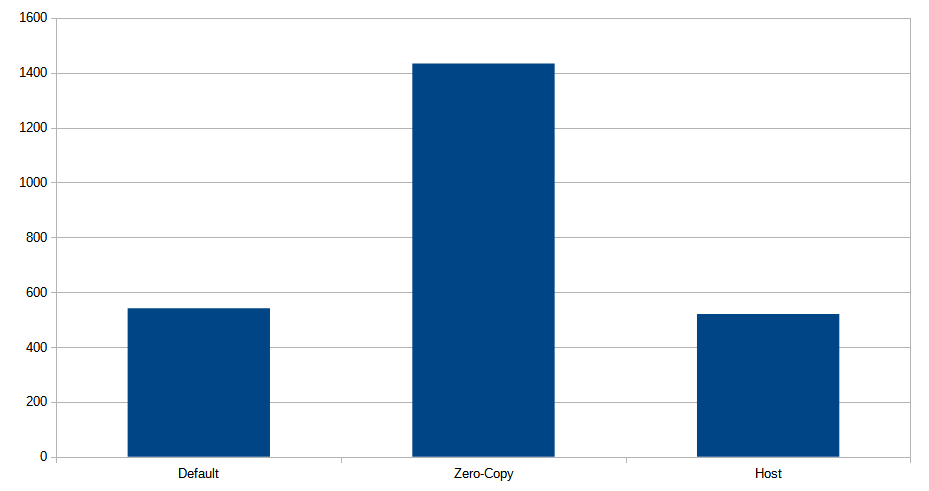
\includegraphics[width=\textwidth]{figures/memory_strategy.png}
    \end{subfigure}
    \hfill
    \caption{Comparison of path finding duration over different memory strategies. Y-axis represents duration in milliseconds. X-axis represents used random seed.}
    \label{fig:mem_strat}
\end{figure*}
%
\section{Conclusion}
%
Creating a fully distributed path-finding solution is very difficult, as pathfinding includes several non-trivial time-distributed data-dependencies, which must be cared for in a clever way.

\begin{itemize}
    \item Use as much debugging as possible, have a macro which allows you to "switch" between debugging and non-debugging mode. Use cudaGetLastError() as much as possible.
    \item Do not rely on intuition when implementing highly parallelized code. Whenever you want to use a mutex, think again.
    \item Try to keep as much data as possible on the GPU and only copy to the CPU if absolutely necessary.
    \item Cuda out of memory errors are prevalent. Try to find a datastructure which fits into your memory conditions.
\end{itemize}
%
\subsection{Improvements Theta* with grid as replacement for priority queue}
%
The following improvements for Theta* with grid would be interesting
\begin{itemize}
    \item Most tiles will most likely not have any occupancy of the algorithm, but the kernel is still being executed for each tile. This could also be improved by applying a prefix sum operator to determine the "occupied" tiles and execute the kernel only on those tiles directly.
    \item Make it work :(
\end{itemize}
%
\subsection{Improvements Theta* with distributed priority queue}
%
The following improvements for Theta* with distributed priority queue would be interesting
\begin{itemize}
    \item Find out why path lengths diverge from sequential implementation
    \item Optimize data structure in memory (cache coherence)
    \item Optimize duplicate detection (no array, instead hashing)
\end{itemize}
\bibliographystyle{plain} % We choose the "plain" reference style
\bibliography{refs} % Entries are in the refs.bib file
%
\end{document}
